\chapter{Polynomial Trajectory Optimization}\label{sec:trajectory}


\section{Polynomial Trajectory}\label{sec:polynomial}

Regarding the differentiability of polynomials, they are a profound choice to represent a trajectory. Especially for the use in a differentially flat representation of the UAV dynamics. (Flatness in the proper sense of system theory means that all the states and inputs can be expressed in terms of the flat output and a finite number of its derivative). \newline
Furthermore, the differentiability of polynomials enables the possibility to check the derivatives of the trajectory for bounding violations to avoid input saturation. This saturation-check can be perform during trajectory optimization and therefore guarantees the feasibility of the resulting trajectory.

\section{Optimization}\label{sec:optimization}

The goal is to optimize a trajectory which passes through way-points (also called vertices or nodes) which are defined in advance. This way-points can be chosen manually or by a path-finding algorithm such as RRT* which will be discussed in Chapter \ref{chap:RRT}.
Furthermore, not only the way-points (therefore the position) can be fixed in advance but also its derivatives (such as speed, acceleration etc.). The position and its derivatives are then utilized as the equality constrains for a QP (explained in Section \ref{sec:quadratic}).

\subsection{Cost Function}\label{sec:cost}

Optimization in terms of trajectory planning means minimization of a cost function. The cost function in this case is a combination of temporal and geometric cost. The geometric cost penalizes the (square) of the derivatives of the trajectory. In this Master Thesis the geometric cost is represented by the squared snap which guarantees a trajectory without abrupt  control inputs. \newline
The temporal cost is simply the total trajectory-time multiplied by a user chosen factor $k_T$ which determines the aggressiveness of the resulting trajectory. \newline

To express the geometric cost in a compact way on can make use of the Hessian matrix $Q$. The Hessian matrix is defined as a squared matrix of second-order partial derivatives which follows from differentiation a function with respect to each of its coefficients (in this instance the polynomial coefficients). The geometric cost function $J(T)$ for a fixed time for one segment can now be written as

\begin{equation}
J(T)  = p^T \cdot Q(T) \cdot p
\end{equation}

where $Q(T)$ is the Hessian matrix for a fixed segment-time $T$ and $p$ is the vector containing the coefficients of the polynomial. \newline

If the trajectory consists of more than one segment the Hessian matrix has to extended to a block-diagonal matrix and the geometric cost function for multiple segments with fixed bud individual segment-times can be written as

\begin{equation}
J =
\begin{bmatrix}
   p_1 \\
\vdots \\
  p_n
\end{bmatrix}^T
\cdot
\begin{bmatrix}
   Q_1(T_1) &  &  \\
    & \ddots &  \\
   & & Q_n(T_n)
\end{bmatrix} 
\cdot
\begin{bmatrix}
   p_1 \\
\vdots \\
  p_n
\end{bmatrix}
\label{equ:cost}
\end{equation}


\subsection{Polynomial Optimization as a Constrained QP}

In a first, intuitive approach the equality constraints on the endpoint derivatives (mentioned in Section \ref{sec:optimization}) are utilized in a constrained QP. Therefore a mapping matrix $E$ between endpoint derivatives and polynomial coefficients is needed. The resulting formula for the $i^{th}$ segment can be written as

\begin{equation}
E_i \cdot p_i = d_i
\label{equ:mapping}
\end{equation}

where $p$ is the vector containing the polynomial coefficients and $d$ is the vector containing the endpoint derivatives. Regarding the total number of segments of the trajectory, Formula \ref{equ:mapping} can be written in matrix form:

\begin{equation}
\begin{bmatrix}
   E_1 &  &  \\
    & \ddots &  \\
   & & E_n
\end{bmatrix} 
\cdot
\begin{bmatrix}
   p_1 \\
\vdots \\
  p_n
\end{bmatrix}
=
\begin{bmatrix}
   d_1 \\
\vdots \\
  d_n
\end{bmatrix}
\end{equation} 

The constrained QP is suitable for a small amount of segments but gets ill-conditioned for a large amount of segments and therefore large matrices. Especially if there are matrices which are close to singularity and have coefficients which are close to zero, the constrained QP can get numerical unstable.

\subsection{Polynomial Optimization as a Unconstrained QP}\label{sec:polynomialQP}

To avoid the numerical instability of a constrained QP the optimization problem is converted into a unconstrained QP. Therefore the polynomial coefficients $p_i$ from Formula \ref{equ:cost} have to be substituted by the endpoint derivatives $d_i$ which are now the new optimizations variables. The cost function of the unconstrained QP can now be written as 

\begin{equation}
J =
\begin{bmatrix}
   d_1 \\
\vdots \\
  d_n
\end{bmatrix}^T
\cdot
\begin{bmatrix}
   E_1 &  &  \\
    & \ddots &  \\
   & & E_n
\end{bmatrix} ^{-T}
\cdot
\begin{bmatrix}
   Q_1 &  &  \\
    & \ddots &  \\
   & & Q_n
\end{bmatrix} 
\cdot
\begin{bmatrix}
   E_1 &  &  \\
    & \ddots &  \\
   & & E_n
\end{bmatrix} ^{-1}
\cdot
\begin{bmatrix}
   d_1 \\
\vdots \\
  d_n
\end{bmatrix}
\label{equ:uncon_cost}
\end{equation}

where $Q_i$ is the Hessian matrix according to the $i^{th}$ segment-time.\newline

As mentioned above, the endpoint derivatives are the new optimization variables. Do to the equality constrains some of the endpoint derivatives are already specified consequently reducing the number of optimizations variables. Expediently, the endpoint derivatives are divided in fixed derivatives $d_f$ and unspecified derivatives $d_p$ and then reordered using the matrix $C$ which consists of zeros and ones. After reordering the endpoint derivatives Formula \ref{equ:uncon_cost} can be rewritten as

\begin{equation}
J =
\begin{bmatrix}
   d_f \\
  d_p
\end{bmatrix}^T
\underbrace{C^T E^{-T} Q E^{-1} C}_\text{R}
\begin{bmatrix}
   d_f \\
  d_p
\end{bmatrix}
\label{equ:R_cost}
\end{equation}

where the product of the reordering matrix $C$, the mapping matrix $E$ and the Hessian matrix $Q$ han be expressed as a single Matrix $R$. The matrix $R$ for his part can be defided into four submatrices according to the fixed and unspecified endpoint derivatives which modifies Formula \ref{equ:R_cost} as follows:

\begin{equation}
J =
\begin{bmatrix}
   d_f \\
  d_p
\end{bmatrix}^T
\begin{bmatrix}
   R_{ff} & R_{fp} \\
  R_{pf} & R_{pp}
\end{bmatrix}
\begin{bmatrix}
   d_f \\
  d_p
\end{bmatrix}
\label{equ:Rxx_cost}
\end{equation}

Partially differenting Formula \ref{equ:Rxx_cost} with respect to the unspecified derivatives $d_p$ and equate it to zero yields the optimized/minimized unspecified derivatives $d_p^*$ 

\begin{equation}
d_p^* = - R_{pp}^{-1} \cdot R_{fp}^T \cdot d_f
\label{equ:dpstar}
\end{equation}

as a function of the fixed derivatives $d_f$ and two of the submatrixes ($R_{pp}, R_{fp}$) of $R$.


\subsection{Initial Solution}\label{sec:initialSolution}

Equation \ref{equ:dpstar} can now be used to compute the initial solution. As can be seen in Equation \ref{equ:uncon_cost} the Hessian matrix for the  $ i^{th}$ segment $Q_i$ depends on the segment-time $i$. Thus, all the segment-times has to be defined. For the initial solution the segment-times are estimated based on the 2-norm distance $d_{norm}$ and on the user specified maximal speed ($v_{max}$) and maximal acceleration ($a_{max}$). \newline
Basically the segment-time is determined by the term $d_{norm}/v_{max} \cdot 2$ which is twice the time the UAV would need for a segment by flying at maximal speed the whole distance. Although this is a good estimation for long segments, for shorter ones the time needed to accelerate gets significant. Therefore a multiplier, which is zero for long segments and unequal to zero for short ones, is added. The segment-time $t_i$ for the $i^{th}$ segment can be computed according to 

\begin{equation}
t_i = \frac{d_{norm_i}}{v_{max}} \cdot 2 \cdot \left( 1 + 6.5 \cdot \frac {v_{max}}{a_{max}} \cdot \frac{1}{e^{\frac{d_{norm_i}}{v_{max}} \cdot 2}} \right)
\label{equ:segmentTime}
\end{equation}

where $d_{norm_i}$ is the 2-norm distance of the $i^{th}$ segment, $v_{max}$ the user specified maximal speed and $a_{max}$ the user specified maximal acceleration. The fraction$v_{max}/a_{max}$ gives an idea how much time is needed to accelerate to max. velocity whereas $6.5$ is a empirical correction factor. \newline

The result from Equation \ref{equ:segmentTime} is depicted in Figure \ref{pic:timeEstimation} whereat the $x$-axis represents the 2-norm distance $d_{norm}$ and the $y$-axis represents the segment time $t$. For this plot the user specified limitation on speed and acceleration has been set to $v_{max} = 3 \frac{m}{s}$ and $a_{max} = 5 \frac{m}{s^2}$. The green line represent the term $d_{norm}/v_{max} \cdot 2$, the blue graph takes the time needed for acceleration into account and is therefore the exact representation of Equation \ref{equ:segmentTime}. \newline


\begin{figure}[h]
   \centering
   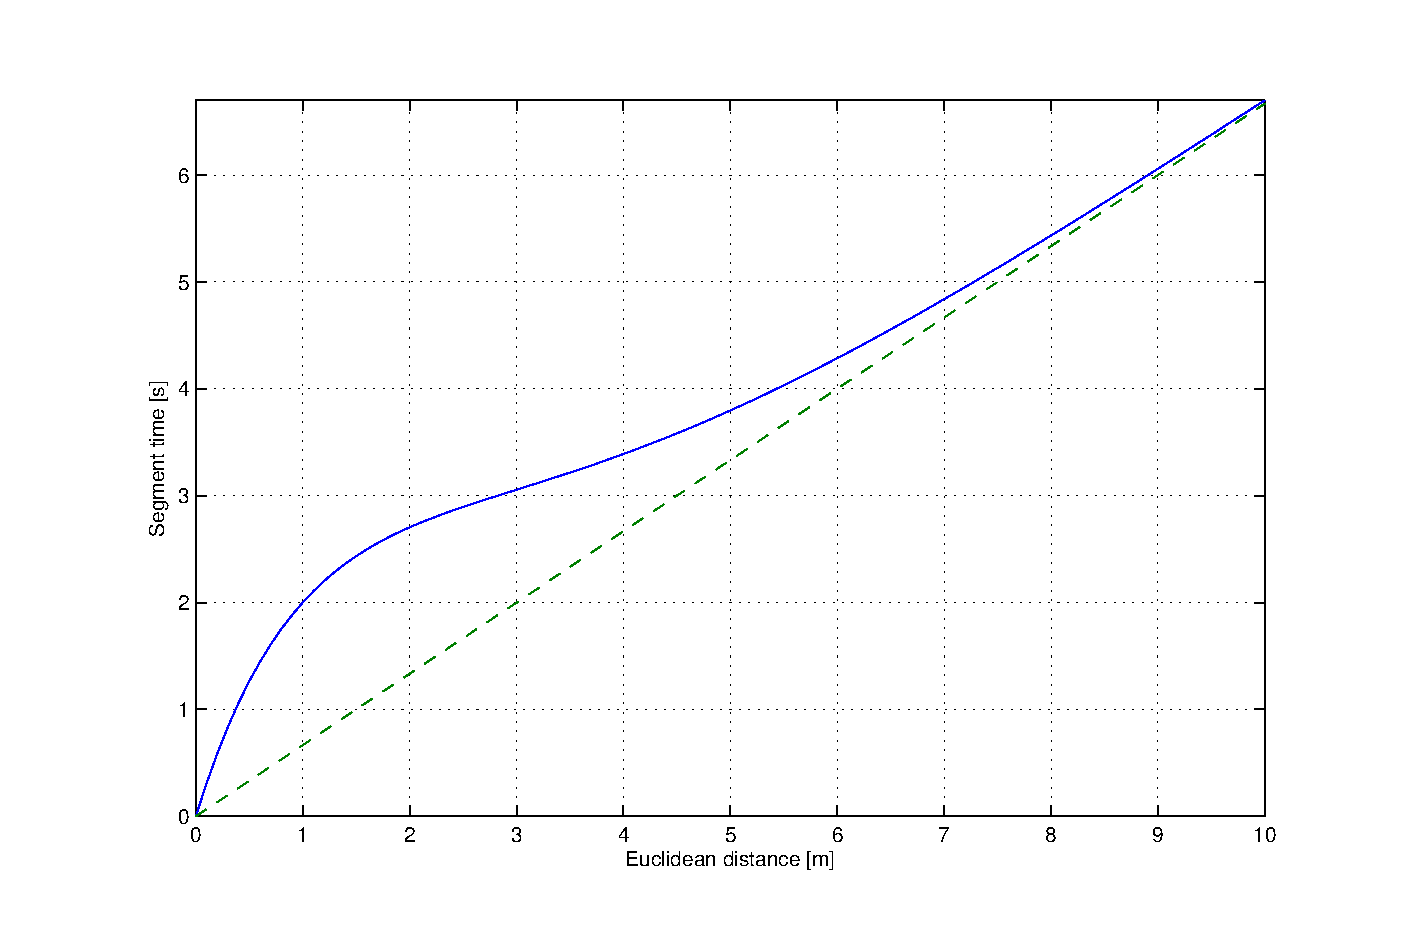
\includegraphics[width=1\textwidth]{pics/time_estimation.eps}
   \caption{The segment-time $t$ depends on the 2-norm distance $d_{norm}$ of a segment and on the maximal speed $v_{max}$ (green line). The blue graph takes  the time needed for acceleration into account and is therefore a more elaborate approach to estimate the segment-time.}
   \label{pic:timeEstimation}
\end{figure}

Once the segment-times are estimated the initial, snap minimized solution can be computed according to Equation \ref{equ:dpstar}. The initial solution for a 3 dimensional problem with 4 segments is depict in Figure \ref{pic:initialSolution}. The first of this 3 subplots shows the position, the second the velocity and the third the acceleration. The $x$-axis for all the 3 subplots is the time. The 3 graphs in the first subplot represent the 3 dimension where the colors are different for each segment. In the second and third subplot, there are also 3 graphs representing a dimension but also a fourth, thicker graph which represents the 2-norm of the velocity respectively the acceleration. Furthermore the limitation ($v_{max} = 3 \frac{m}{s}$ and $a_{max} = 2 \frac{m}{s^2}$ for this problem) are depicted.

\subsection{Penalty on Time}\label{sec:penalty}

So fare, only the geometric cost (i. e. the squared snap) was discussed. Minimization of the geometric cost ensures a smooth trajectory without abrupt input signal but has no effect on the aggressiveness of a trajectory. Therefore Formula \ref{equ:Rxx_cost} has to be extended by the temporal cost which results in the total cost $J_{total}$:

\begin{equation}
J_{total} =
\begin{bmatrix}
   d_f \\
  d_p
\end{bmatrix}^T
\begin{bmatrix}
   R_{ff} & R_{fp} \\
  R_{pf} & R_{pp}
\end{bmatrix}
\begin{bmatrix}
   d_f \\
  d_p
\end{bmatrix}
+ k_T \cdot \sum_{i=1}^N T_i
\label{equ:total_cost}
\end{equation}

where $k_T$ is a user specified penalty on time and $T_i$ is the segment-time of the $i^{th}$ segment.

\begin{figure}[h]
   \centering
   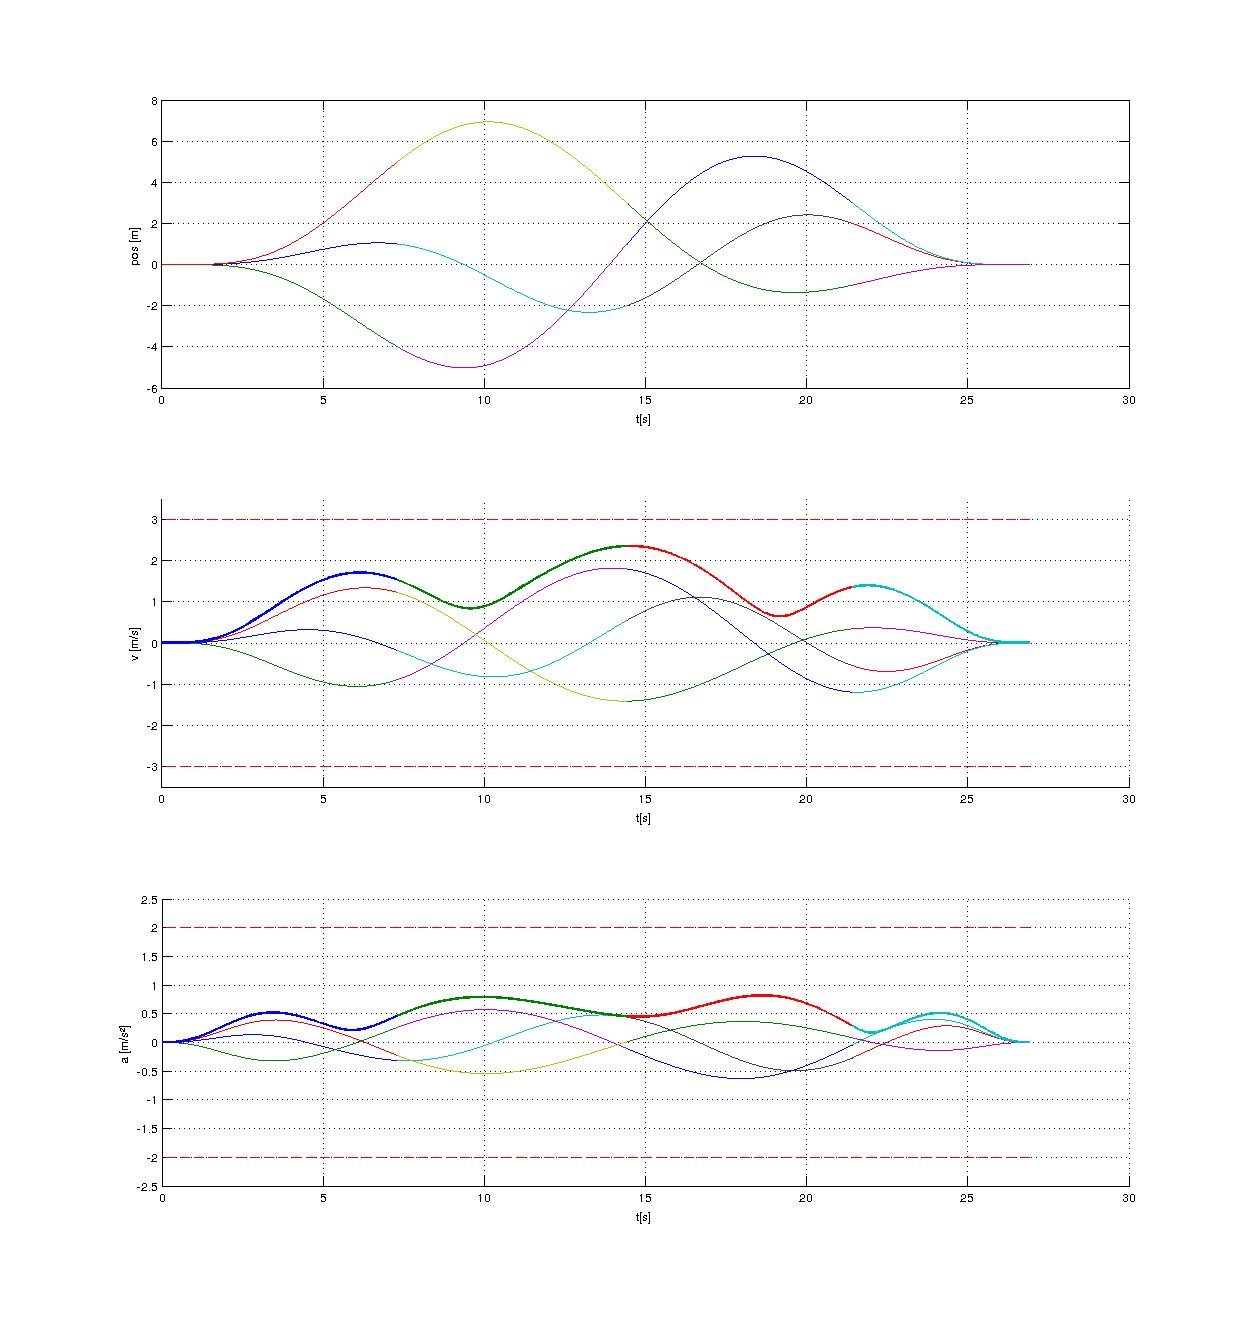
\includegraphics[width=1\textwidth]{pics/initial.jpg}
   \caption{Initial solution: The first subplot shows the position, the second the velocity and the third the acceleration of the initial solution. A thicker graph represents the 2-norm of the velocity respectively the acceleration.}
   \label{pic:initialSolution}
\end{figure}

In contrast to Equation \ref{equ:Rxx_cost}, Equation \ref{equ:total_cost} cannot be solved analytically. Due to that a nonlinear solver is used. In this thesis NLopt,  a open-source library for nonlinear optimization, is applied. The optimizations variables of the nonlinear optimization are the estimated segment-times and the unspecified endpoint derivatives $dp$. The computational cost of the nonlinear optimization is highly depending on the quality of the initial solution. \newline
The termination condition of the optimization can be specified on the optimization variables as well as on the total cost. Generally, the termination conditions are formulated relative to the current value(s). For instance, if the relative termination condition for the total cost $J_{rel}$ is set to $0.01$ the optimization ends if the total cost changes less than a percent during a iteration. The relative termination condition for the optimization variables $x_{rel}$ is only fulfilled if all of the optimization variables change less then the threshold. Additionally, a absolute termination condition $x_{abs}$ is applied to the optimization variables but is only called into action if one or several optimization variables are close to zero and the relative criteria therefore don't work properly.
During the optimization the constraints on velocity and acceleration are checked every iteration. \newline

The result of the nonlinear optimization is depicted in Figure \ref{pic:optimizedSolution}. As can be seen, the trajectory passing the same way-points as in Figure \ref{pic:initialSolution} only needs around 18 seconds where as the initial solution required around 27 second. 



\begin{figure}[h]
   \centering
   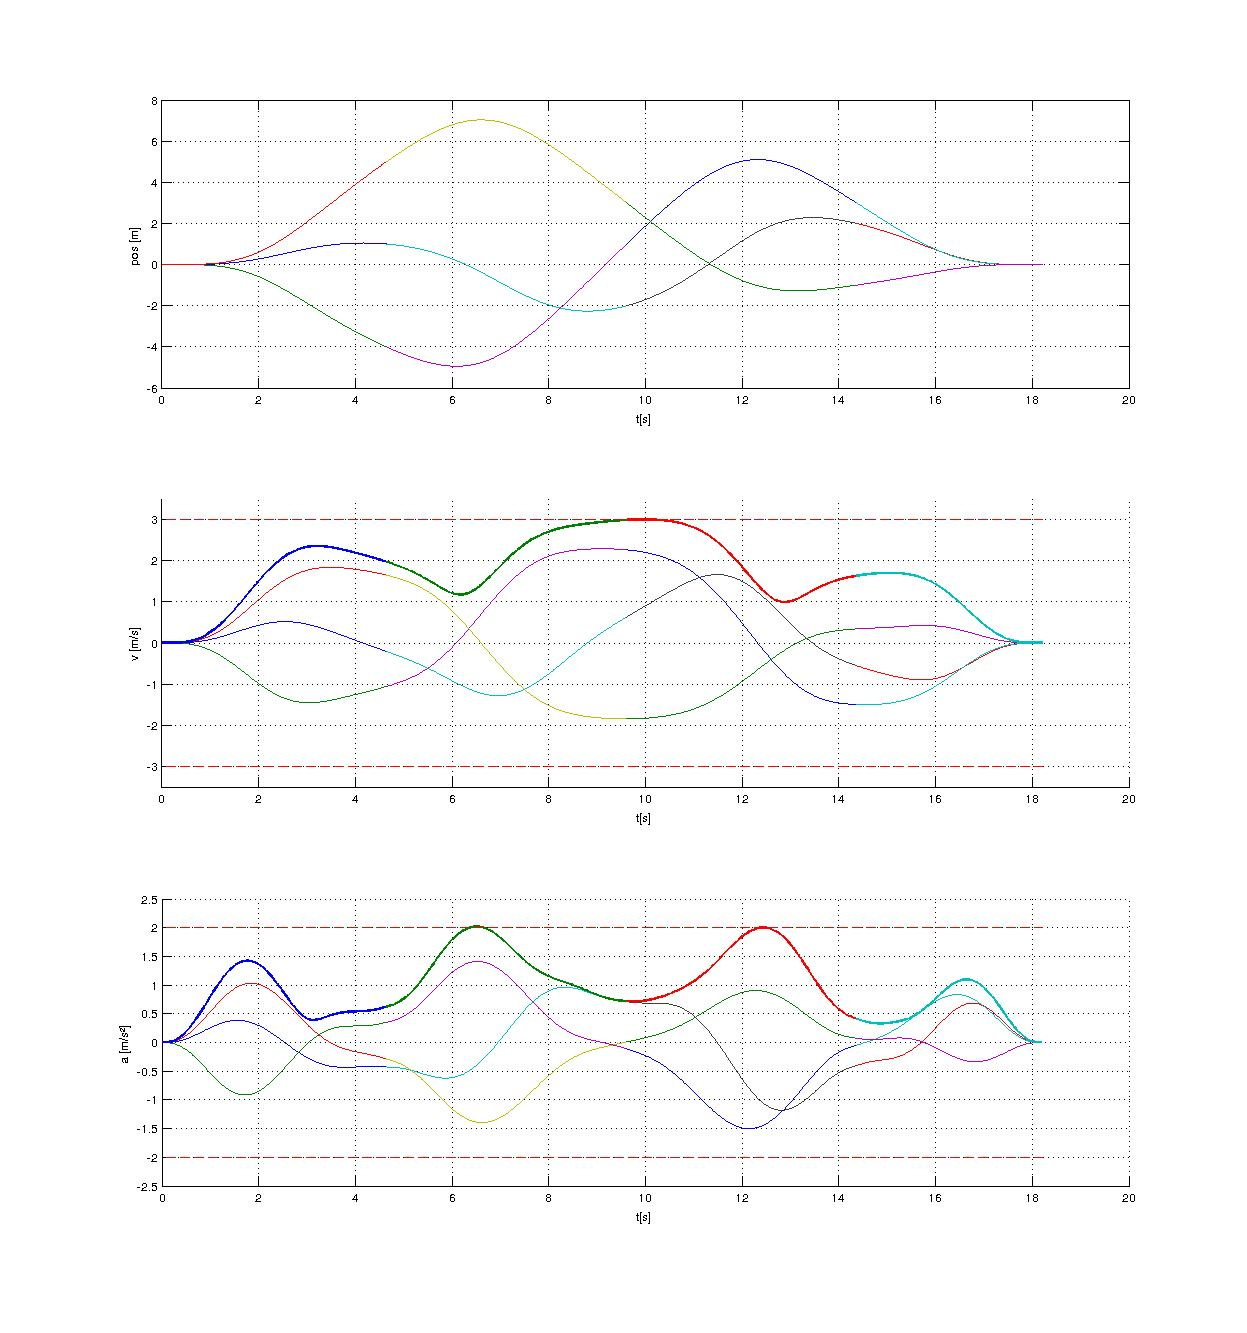
\includegraphics[width=1\textwidth]{pics/optimized.jpg}
   \caption{Optimized solution: The first subplot shows the position, the second the velocity and the third the acceleration of the optimized solution. A thicker graph represents the 2-norm of the velocity respectively the acceleration. }
   \label{pic:optimizedSolution}
\end{figure}

%\begin{figure}[h]
%   \centering
%   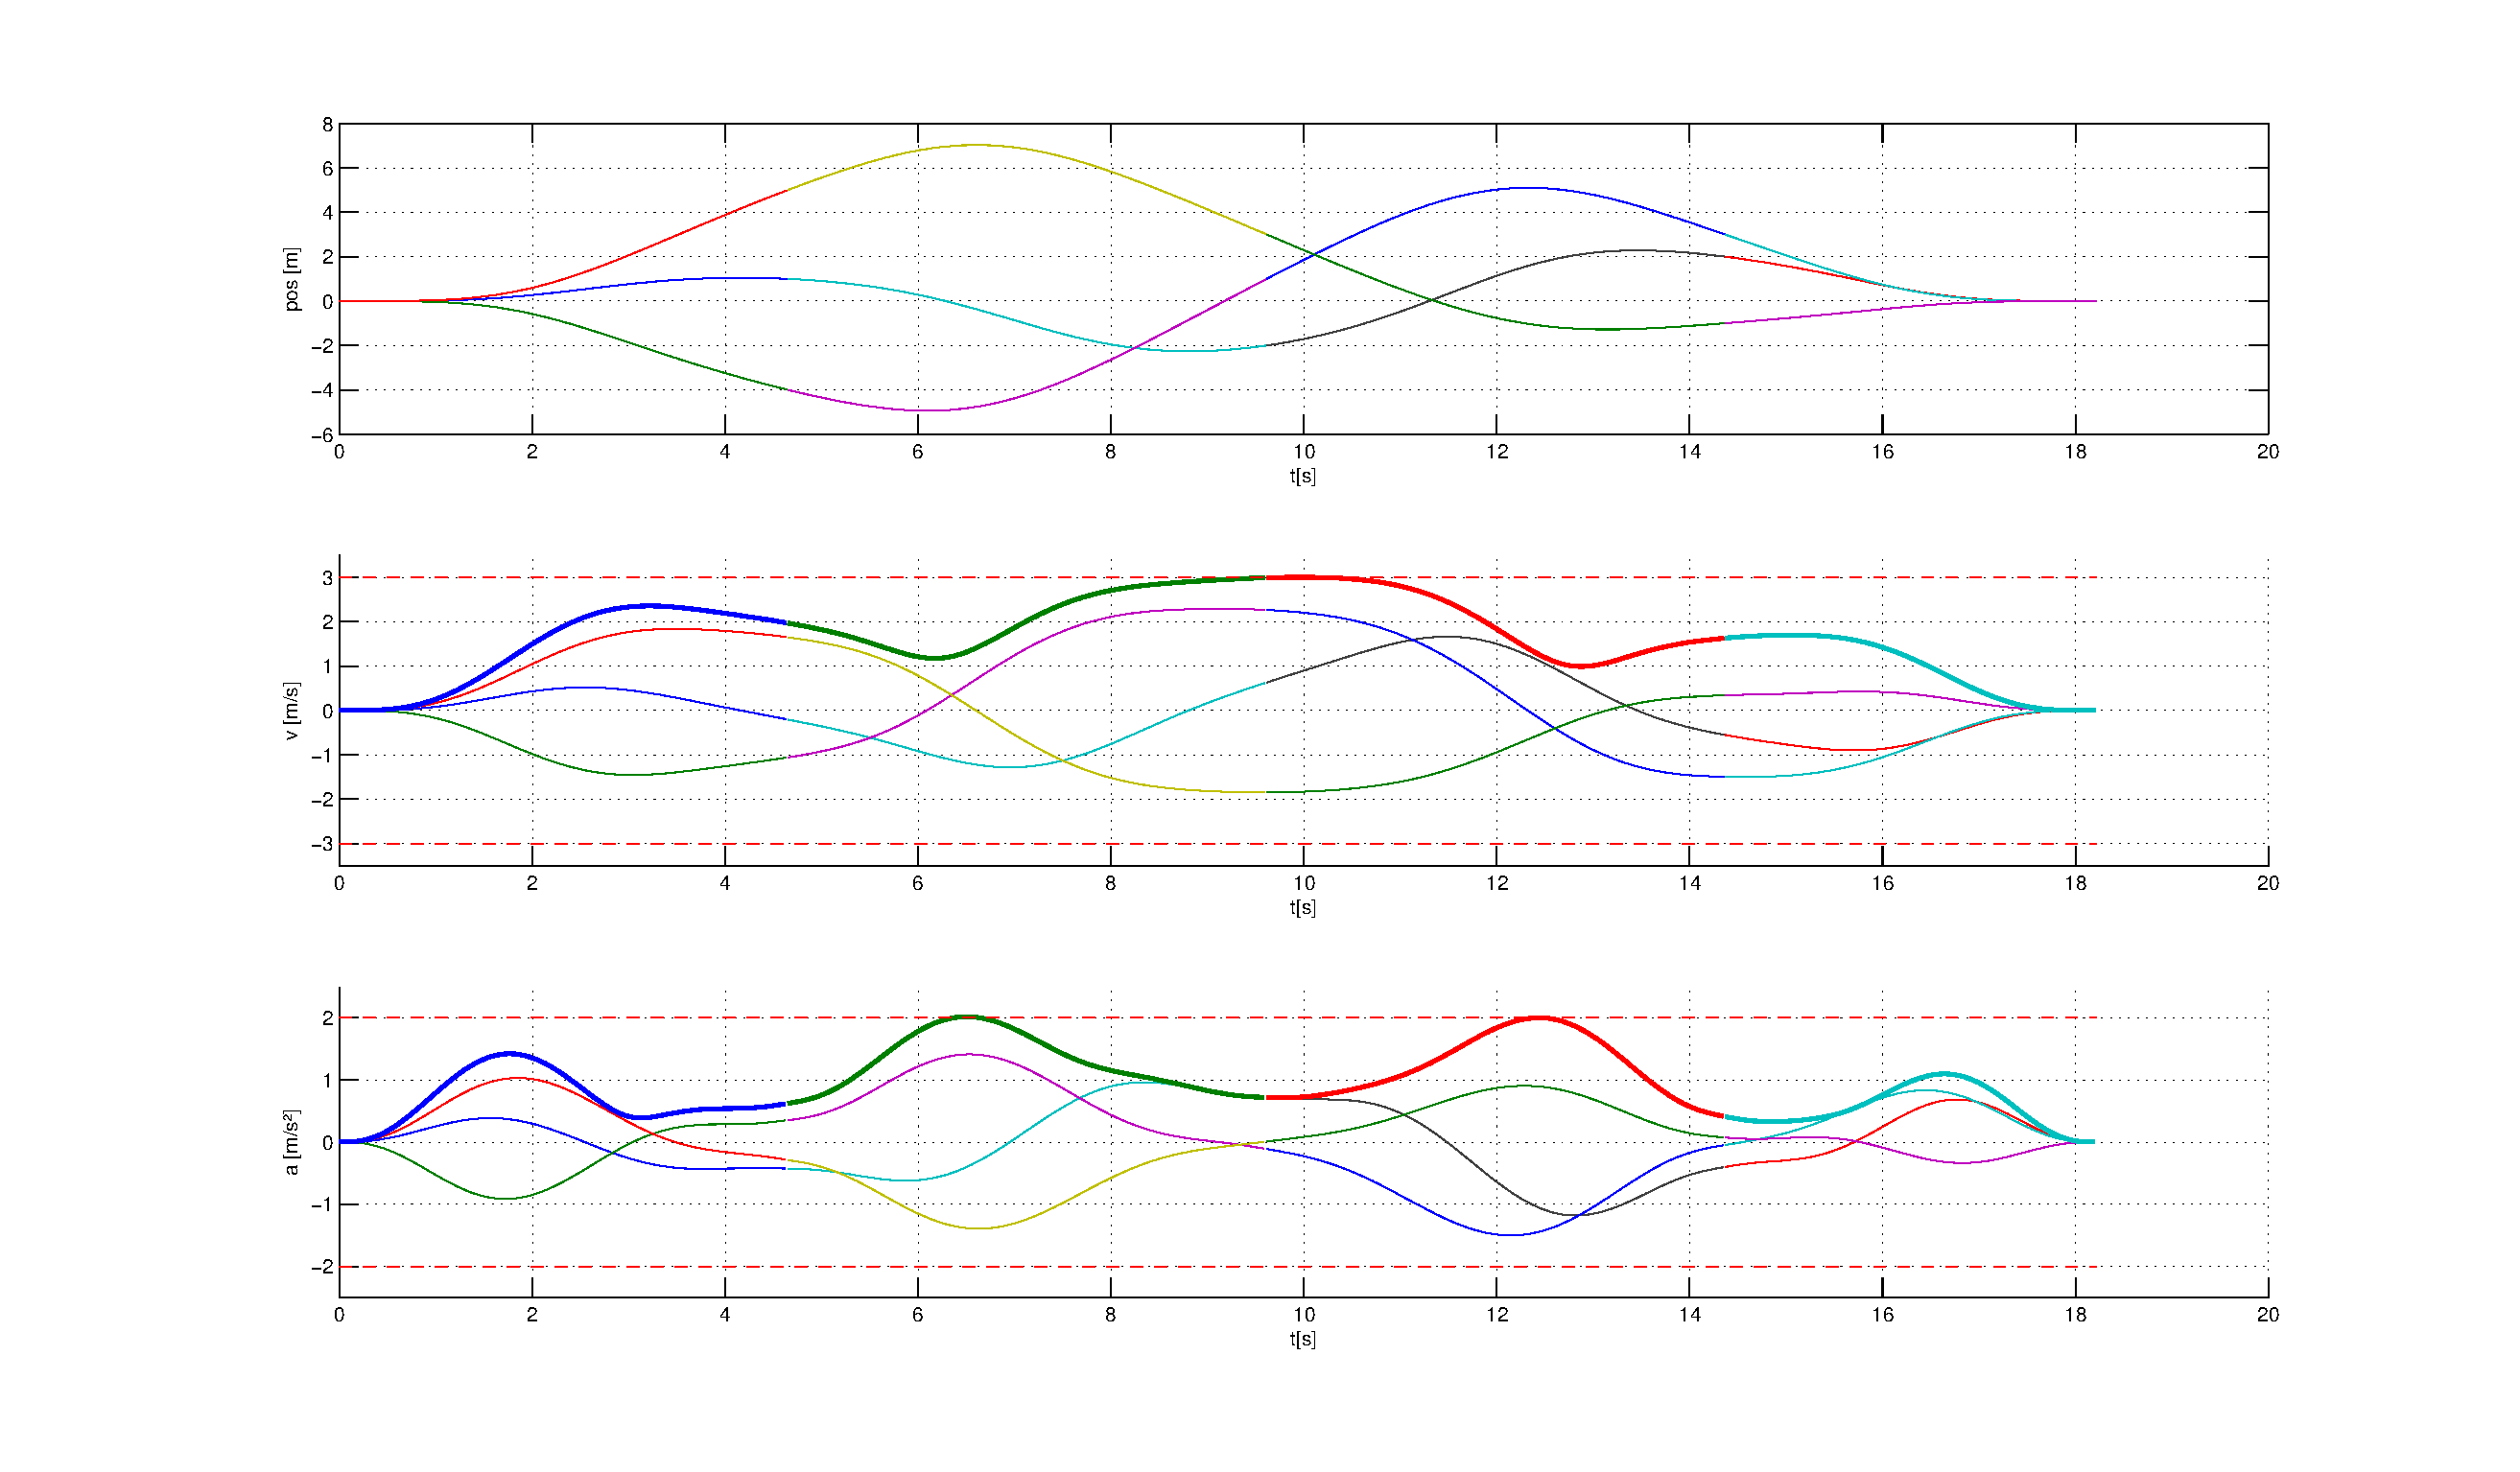
\includegraphics[width=1\textwidth]{pics/optimized.eps}
%   \caption{Ein Bild.}
%\end{figure}
%
%
%\begin{figure}[h]
%   \centering
%   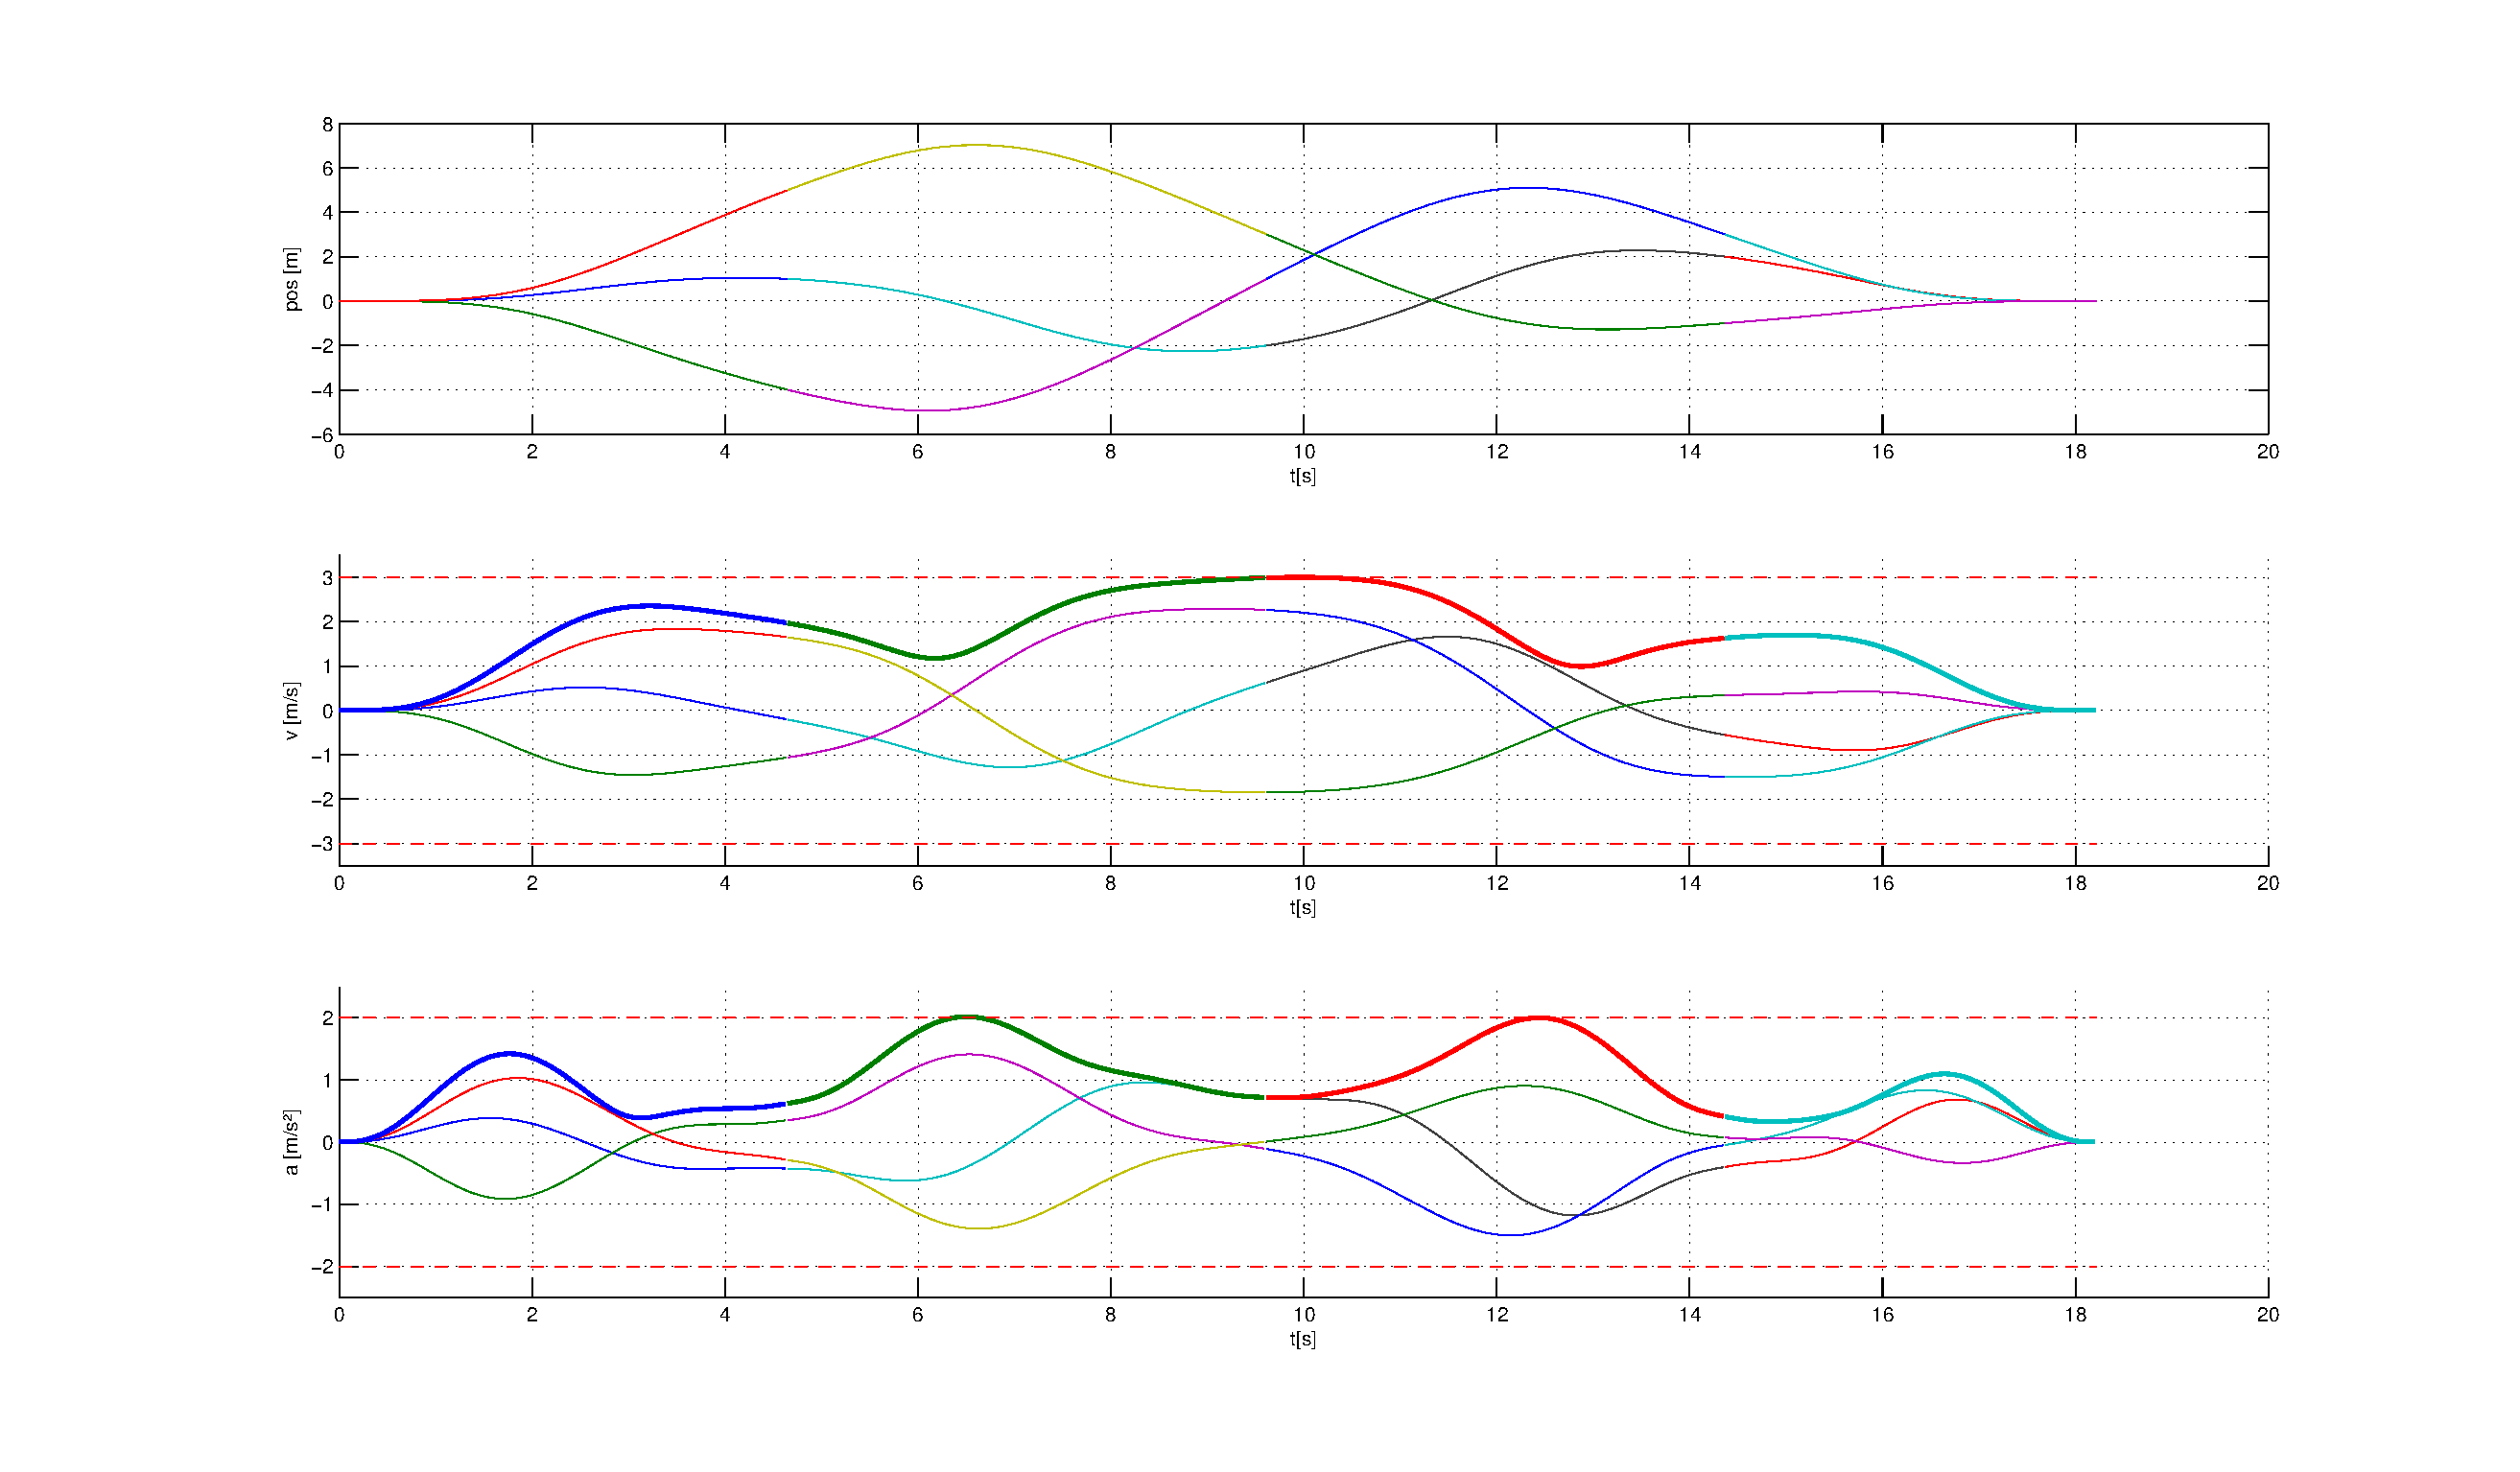
\includegraphics[scale=0.3]{pics/optimized.eps}
%   \caption{Ein Bild.}
%\end{figure}



%\begin{figure}[h]
%   \centering
%   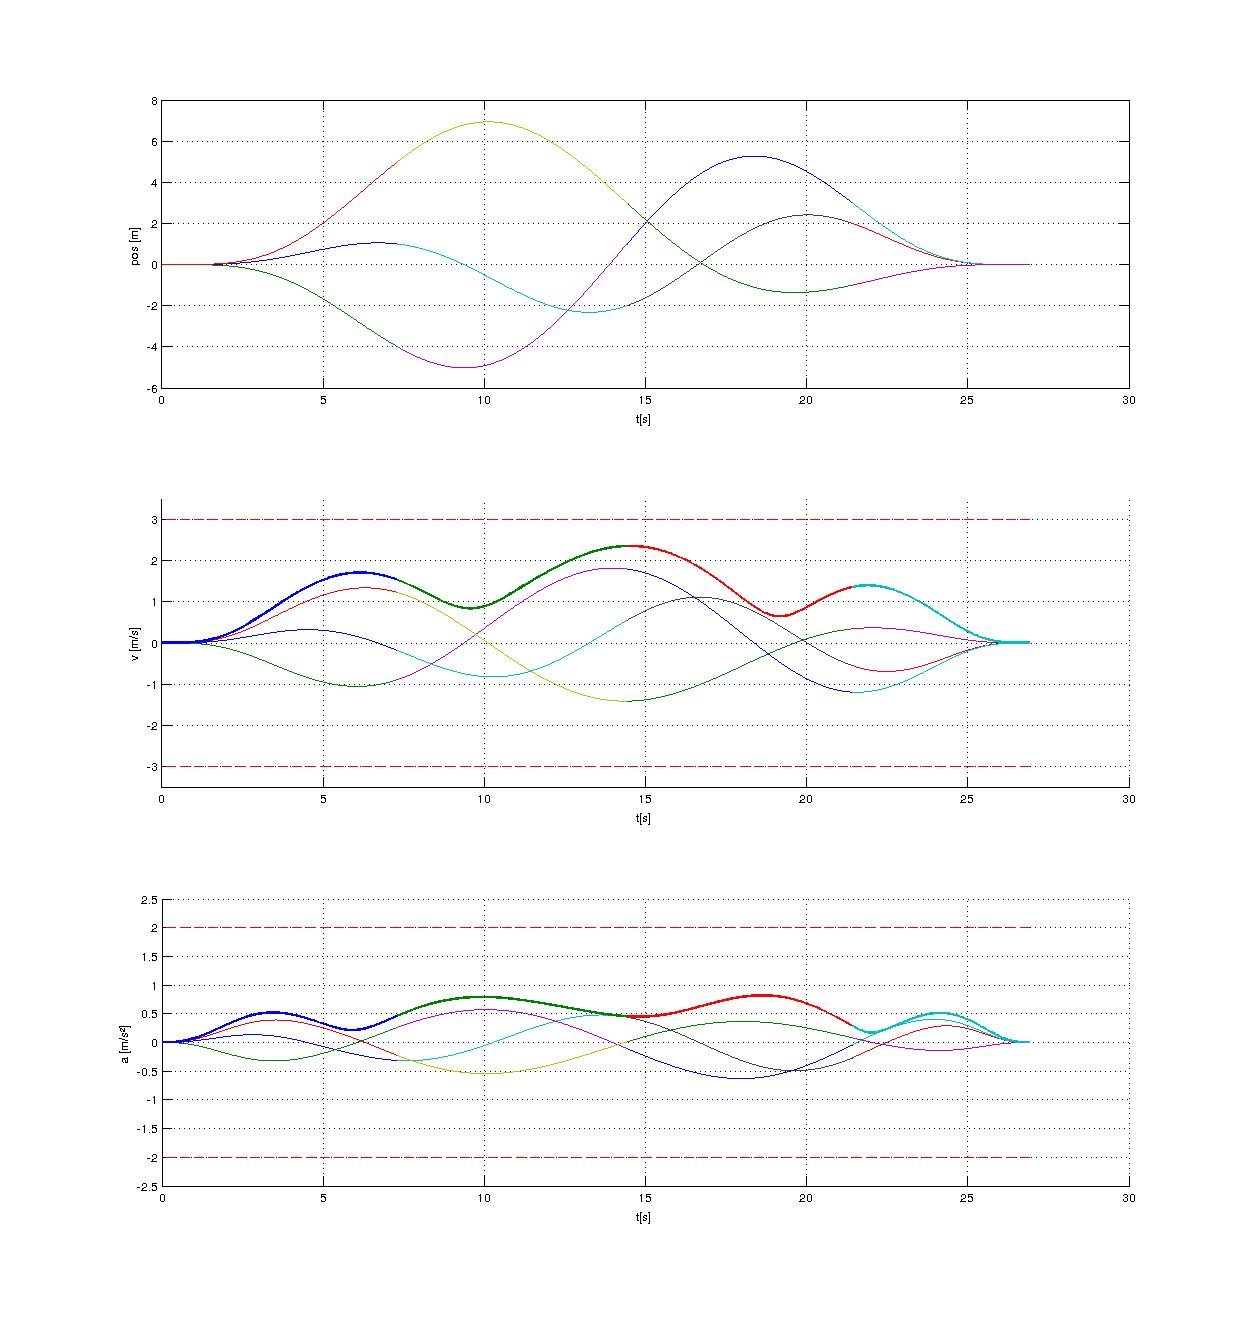
\includegraphics[width=1\textwidth]{pics/initial.eps}
%   \caption{Ein Bild.}
%\end{figure}

%\begin{figure}[h]
%   \centering
%   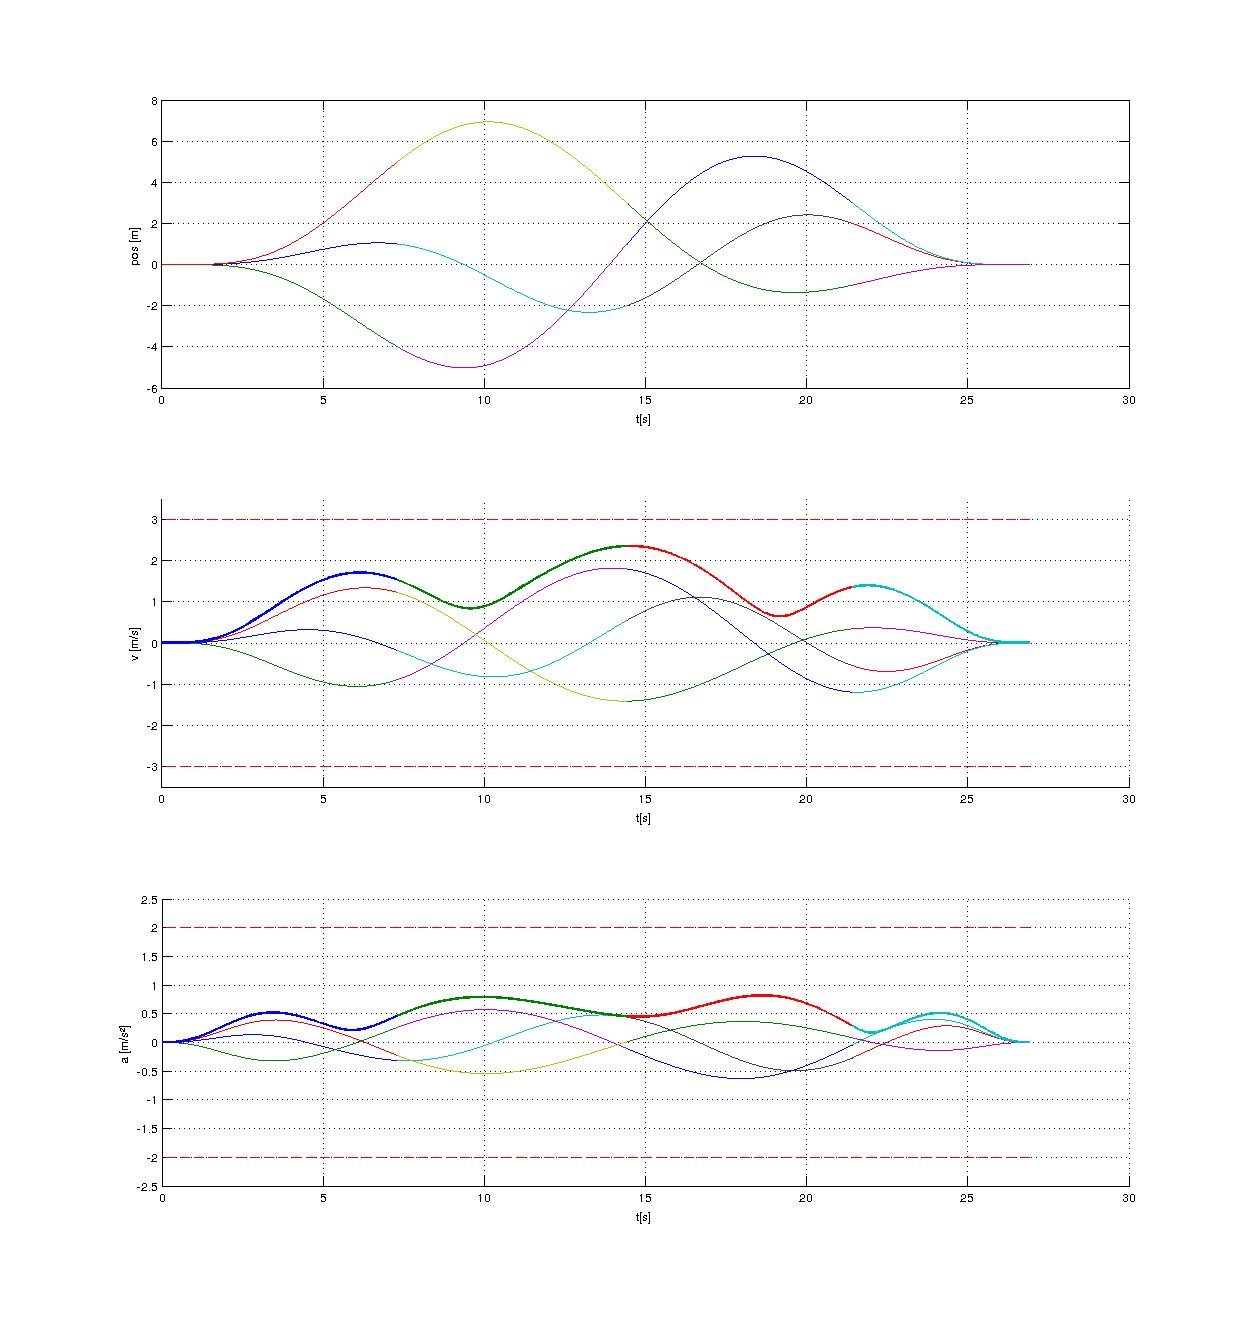
\includegraphics[scale=1]{pics/initial.eps}
%   \caption{Schematic of a rough foot surface.}
%   \label{pics:profile2}
%\end{figure}























